\section{Architektur}
Nun gilt es das in Kapitel \ref{sec:konzept} vorgestellte Konzept umzusetzen. Dazu haben wir eine Architektur für einen Sprachassistenten entwickelten, welche in Abbildung \ref{fig:infrastruktur-overview} zu sehen ist. Diese Architektur soll mehr Privatsphäre bieten und unterteilt sich in drei Hauptmodul: die mobile App, das Repository und die Cloud. Was auffällt, das es zweimal das Untermodul "Speech Processing" gibt. Dabei wird in der mobilen App einfache Sprachverarbeitung wie beispielsweise das Aufnehmen bzw. die Wiedergabe eines Audiofiles implementiert. Ressourcen intensive Sprachverarbeitungsprozesse wie beispielsweise die Umwandlung von Sprache zu Text werden in die Cloud ausgelagert. Im folgenden werden die drei Hauptmodule genauer beschrieben.
\begin{figure}[h!]
	\centering
	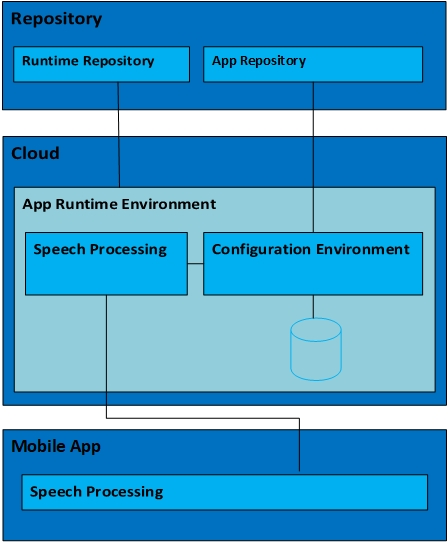
\includegraphics[width=0.9\linewidth]{Picture/Infrastruktur-Overview.jpg}
	\caption[Architektur Übersicht]{Architektur Übersicht}
	\label{fig:infrastruktur-overview}
\end{figure}

\subsection{mobile App}
Die mobile App ist die Schnittstelle zum Nutzer und wie Abbildung \ref{fig:infrastruktur-app} zeigt, hat diese drei Aufgaben:

\begin{itemize}
	\item \textsl{Speech Recording:} Aufnehmen und streamen der Eingabe eines Nutzers an die Cloud.
	\item \textsl{Speech Playback:} Abspielen eines Streams, der von der Cloud erzeugt wurde.
	\item \textsl{Hotword Detection:} Die mobile App soll nicht ununterbrochen die Eingabe des Nutzers aufnehmen und streamen, denn diese könnte die Privatsphäre des Nutzer beeinträchtigen. Die App soll nur aufnehmen und streamen, wenn der Nutzer das will. Somit kommt die sogenannte "Hotword Detection" zum Einsatz. Dies belauscht den Nutzer durchgängig, jedoch nur lokal auf dem Endgerät und ohne Daten via Internetverbindung weiter zu senden. Eine Hotword Detection benötigt kaum Ressourcen, da sie für die Erkennung eines einzigen Signalwortes optimiert wurde. Somit lässt sich ein Signalwort definieren, sobald der Nutzer dieses Signalwort sagt, wird das Aufnehmen und streamen an die Cloud gestartet.
\end{itemize}

Die mobile App soll auf verschiedenen mobilen Plattform wie Android, iOS, Windows Phone und als Webanwendung implementiert werden. Des Weiteren wäre auch die Integration der mobilen App in einen Lautsprecher eine Überlegung wert.

\begin{figure}[h!]
	\centering
	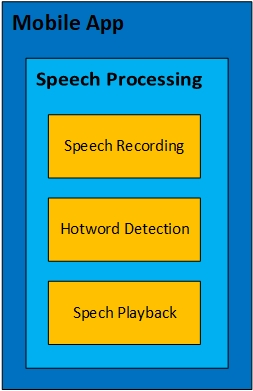
\includegraphics[width=0.3\linewidth]{Picture/Infrastruktur-App.jpg}
	\caption[Architektur - mobile App]{Architektur - mobile App}
	\label{fig:infrastruktur-app}
\end{figure}

\subsection{Repository}
Das Repository unterteilt sich nochmal in zwei 
\begin{figure}[h!]
	\centering
	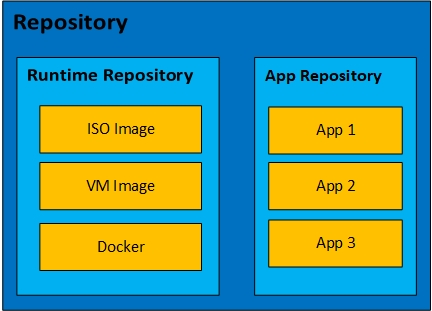
\includegraphics[width=0.6\linewidth]{Picture/Infrastruktur-Repository.jpg}
	\caption[Architektur - mobile App]{Architektur - Repository}
	\label{fig:infrastruktur-repository}
\end{figure}

\subsection{Cloud}
Die Cloud
\begin{figure}[h!]
	\centering
	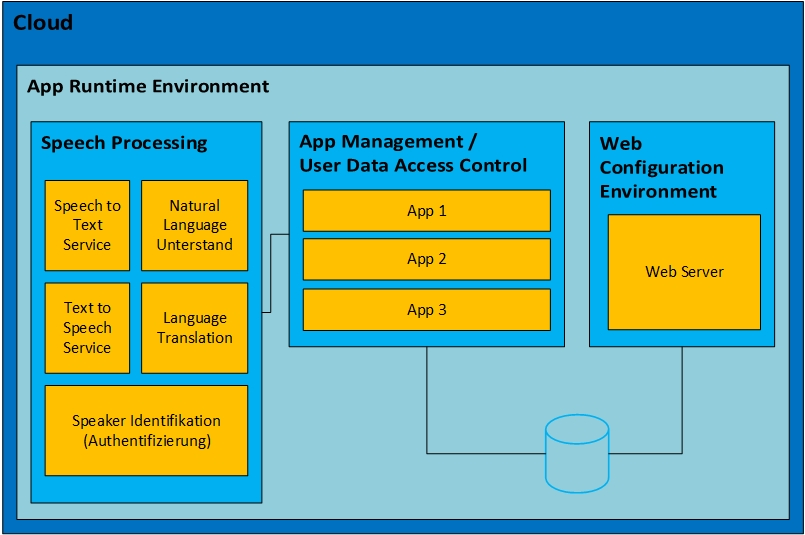
\includegraphics[width=0.9\linewidth]{Picture/Infrastruktur-Cloud.jpg}
	\caption[Architektur - mobile App]{Architektur - Cloud}
	\label{fig:infrastruktur-cloud}
\end{figure}





